\documentclass[tikz,border=10pt]{standalone}
\usepackage{tikz}
\usetikzlibrary{arrows.meta, positioning, shapes.geometric, fit, backgrounds}

\begin{document}
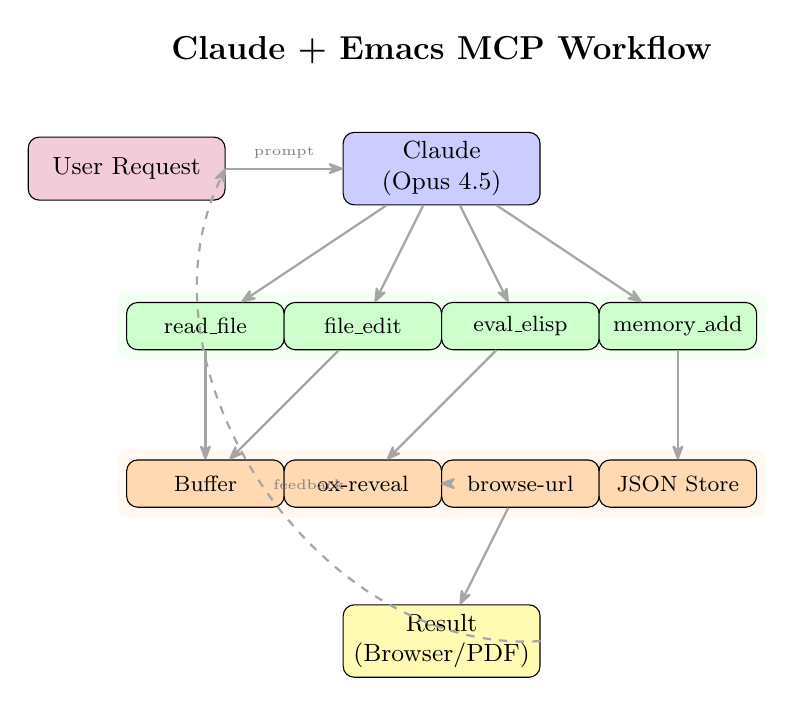
\begin{tikzpicture}[
    node distance=1.5cm,
    >={Stealth[round]},
    box/.style={rectangle, rounded corners, draw=black, fill=blue!20, 
                minimum width=2.5cm, minimum height=0.8cm, align=center, font=\small},
    tool/.style={rectangle, rounded corners, draw=black, fill=green!20,
                minimum width=2cm, minimum height=0.6cm, align=center, font=\footnotesize},
    emacs/.style={rectangle, rounded corners, draw=black, fill=orange!30,
                minimum width=2cm, minimum height=0.6cm, align=center, font=\footnotesize},
    arrow/.style={->, thick, draw=gray!70},
    label/.style={font=\tiny, text=gray}
]

% Title
\node[font=\large\bfseries] at (4, 4) {Claude + Emacs MCP Workflow};

% User
\node[box, fill=purple!20] (user) at (0, 2.5) {User Request};

% Claude Processing
\node[box] (claude) at (4, 2.5) {Claude\\(Opus 4.5)};

% Tools Layer
\node[tool] (read) at (1, 0.5) {read\_file};
\node[tool] (edit) at (3, 0.5) {file\_edit};
\node[tool] (eval) at (5, 0.5) {eval\_elisp};
\node[tool] (memory) at (7, 0.5) {memory\_add};

% Emacs Layer
\node[emacs] (buffer) at (1, -1.5) {Buffer};
\node[emacs] (export) at (3, -1.5) {ox-reveal};
\node[emacs] (browser) at (5, -1.5) {browse-url};
\node[emacs] (memstore) at (7, -1.5) {JSON Store};

% Output
\node[box, fill=yellow!30] (output) at (4, -3.5) {Result\\(Browser/PDF)};

% Arrows - User to Claude
\draw[arrow] (user) -- (claude) node[midway, above, label] {prompt};

% Claude to Tools
\draw[arrow] (claude) -- (read) node[midway, left, label] {};
\draw[arrow] (claude) -- (edit);
\draw[arrow] (claude) -- (eval);
\draw[arrow] (claude) -- (memory);

% Tools to Emacs
\draw[arrow] (read) -- (buffer);
\draw[arrow] (edit) -- (buffer);
\draw[arrow] (eval) -- (export);
\draw[arrow] (memory) -- (memstore);

% Emacs to Output
\draw[arrow] (export) -- (browser);
\draw[arrow] (browser) -- (output);

% Feedback loop
\draw[arrow, dashed, bend left=60] (output.east) to node[right, label] {feedback} (user.east);

% Background groups
\begin{scope}[on background layer]
    \node[fit=(read)(edit)(eval)(memory), fill=green!5, rounded corners, 
          label={[font=\footnotesize]above:MCP Tools}] {};
    \node[fit=(buffer)(export)(browser)(memstore), fill=orange!5, rounded corners,
          label={[font=\footnotesize]below:Emacs}] {};
\end{scope}

\end{tikzpicture}
\end{document}
